\documentclass[noauthor, nooutcomes]{ximera}

\input{../preamble.tex}
\author{Elizabeth Miller}
\license{Creative Commons Attribution-ShareAlike 4.0 International License}
\acknowledgement{https://spot.pcc.edu/math/orcca/ed2/html/section-technical-definition-of-a-function.html, https://activecalculus.org/prelude/sec-changing-functions-models.html, https://openstax.org/books/college-algebra/pages/3-1-functions-and-function-notation}

\title{What is a Function?}

\begin{document}
\begin{abstract}
  
\end{abstract}
\licenseAPCSZORCCA
\maketitle


%\typeout{************************************************}
%\typeout{Motivating Questions}
%\typeout{************************************************}

\begin{motivatingQuestions}\begin{itemize}
\item What is a function?
\item How can functions be represented?
\item When is a relation not a function?
\end{itemize}\end{motivatingQuestions}


%\typeout{************************************************}
%\typeout{Subsection Introduction}
%\typeout{************************************************}

\section{Mathematical Models}
A mathematical model is an abstract concept through which we use mathematical language and notation to describe a phenomenon in the world around us.  One example of a mathematical model is found in \link[Dolbear's Law,]{https://en.wikipedia.org/wiki/Dolbear\%27s_law} which has proven to be remarkably accurate for the behavior of snowy tree crickets.  For even more of the story, including a reference to this phenomenon on the popular show The Big Bang Theory, see \link{https://priceonomics.com/how-to-tell-the-temperature-using-crickets/}.  In the late 1800s, the physicist Amos Dolbear was listening to crickets chirp and noticed a pattern: how frequently the crickets chirped seemed to be connected to the outside temperature.  

\begin{image}
\includegraphics[width=.8\textwidth]{CompositionText3.jpg}
\end{image}

If we let $T$ represent the temperature in degrees Fahrenheit and $N$ the number of chirps per minute, we can summarize Dolbear's observations in the following table.

$$
\begin{array}{cc}
N \text{(chirps per minute)} & T \text{(degrees Fahrenheit)}\\
\hline
40&50\\
80&60\\
120&70\\
160&80
\end{array}
$$

For a mathematical model, we often seek an algebraic formula that captures observed behavior accurately and can be used to predict behavior not yet observed.  For the data in the table above, we observe that each of the ordered pairs in the table make the equation%
\begin{equation*}
T = 40 + 0.25N
\end{equation*}
true.  For instance, $70 = 40 + 0.25(120)$.  Indeed, scientists who made many additional cricket chirp observations following Dolbear's initial counts found that the formula above holds with remarkable accuracy for the snowy tree cricket in temperatures ranging from about $50^\circ$ F to $85^\circ$ F.

This model captures a pattern that is found in the world, and can be used to predict the temperature if only the number of chirps per minute is known.  Not all phenomenon in the world that can be measured mathematically occur in a predictable pattern.  In this section, we will study functions which are mathematical ways of formally studying situations where for a given input, such as the number of chirps above, there is one consistant output.  For situations where a given input might give a variety of outputs, we encourage you to study statistics! Also note that this relationship is not causal. Even though the number of chirps is considered out ``input'' the increase in chirps does not cause the temperature to increase. 

\section{Functions}
The mathematical concept of a function is one of the most central ideas in all of mathematics, in part since functions provide an important tool for representing and explaining patterns.  At its core, a function is a repeatable process that takes a collection of input values and generates a corresponding collection of output values with the property that if we use a particular single input, the process always produces exactly the same single output.

For instance, Dolbear's Law provides a process that takes a given number of chirps between $40$ and $180$ per minute and reliably produces the corresponding temperature that corresponds to the number of chirps, and thus this equation generates a function.  We often give functions shorthand names; using ``$D$'' for the ``Dolbear'' function, we can represent the process of taking inputs (observed chirp rates) to outputs (corresponding temperatures) using arrows:%
\begin{align*}
80 &\xrightarrow{D} 60\\
120 &\xrightarrow{D} 70\\
N &\xrightarrow{D} 40 + 0.25 N
\end{align*}

Alternatively, for the relationship ``$80 \xrightarrow{D} 60$'' we can also use the equivalent notation ``$D(80) = 60$'' to indicate that Dolbear's Law takes an input of $80$ chirps per minute and produces a corresponding output of $60$ degrees Fahrenheit.  More generally, we write ``$T = D(N) = 40 + 0.25N$'' to indicate that a certain temperature, $T$, is determined by a given number of chirps per minute, $N$, according to the process $D(N) = 40 + 0.25N$.


We will define a function informally and formally.  The informal definition corresponds to the way we will most often think of functions, as a process with inputs and outputs.  

\begin{definition}[Informal Definition of a Function]
A \dfn{function} is a process that may be applied to a collection of input values to produce a corresponding collection of output values in such a way that the process produces one and only one output value for any single input value.
\end{definition}

The formal definition of a function will establish a function as a special type of relation.  Recall that a \emph{relation} is a collection of points of the form $(x,y)$.  If the point $(x_0,y_0)$ is in the relation, then we say $x_0$ and $y_0$ are \emph{related}.

\begin{definition}[Formal Definition of a Function]
A \dfn{function} is a collection of ordered pairs $(x,y)$ such that any particular value of $x$ is paired with at most one value for $y$. That is, a relation in which each $x$-coordinate is matched with only one $y$-coordinate is said to describe $y$ as a \dfn{function} of $x$.
\end{definition}

How is this definition consistent with the informal, which describes a function as a process? Well, if you have a collection of ordered pairs $(x,y)$, you can choose to view the left number as an input, and the right value as the output. If the function's name is $f$ and you want to find $f(x)$  for a particular number $x$, look in the collection of ordered pairs to see if $x$ appears among the first coordinates. If it does, then $f(x)$ is the (unique) $y$-value it was paired with. If it does not, then that $x$ is just not in the domain of $f$, because you have no way to determine what $f(x)$ would be.

\section{Respresentations of Functions}
While the formal definition of a function is a set of ordered pairs, there are many ways that we represent functions when studying them.  Each representation has advantages and disadvantages and being able to change between different representations of the same function is an important skill.  Let's look at some different types of representations.

\subsection{Tables}
Functions on a finite set of points are often represented by tables.  One advantage of a table is that you can easily see all the information for a function.  One disadvantage is if you have too many input values, it can be difficult to analyze them all in a table format.  The exploration below shows and example of a function given by a table.

\begin{exploration}
The function $f$ is defined by the table below. Note: this means the table gives all the values of the function.\\ 
Answer the questions about the function below.

$$
\begin{array}{cc}
x & f(x) \\
\hline
\text{banana}&.5\\
\text{apple}&1.59\\
\text{pear}&2.50\\
\text{orange}&1
\end{array}
$$

\begin{enumerate}[label=\alph*.]
\item Is $f$ a function? 
\item What is $f(\text{apple})$?
\item  What are the inputs of $f$?
\item  What are the outputs of $f$?
\item Rewrite $f$ as a set of ordered pairs.
\item  Assume that $f$ gives the price of a single item of a given fruit at a grocery store.  Interpret $f(\text{orange})=1$ in this context.
\end{enumerate}
\end{exploration}

If the set of ordered pairs that makes up your function is an infinite set, you cannot represent your entire function as a table because it would go on forever!  Instead, you might see a table with a sampling of points from a function. In that case, unless you have additional information about your function, you cannot know what the outputs are for inputs not listed in the table.  In fact, without additional information, you cannot even say which values are allowed to be inputs for the function!

\subsection{Arrow Diagrams}
Arrow diagrams are another tool used to represent functions.  Here is an arrow diagram that corresponds to the function $f$ in the exploration above.

\begin{image}
\includegraphics{WiaF-arrowDiagram.pdf}
\end{image}

Arrow diagrams can help make it easier to see when multiple inputs go to the same output.  Arrow diagrams can also be used to represent relations, and can make it easier to see if the relation is a function. The three arrow diagrams below show relations.  The first two relations are functions, but the last relation is not a function because the same input goes to two different outputs.

\begin{image}
\includegraphics[width=\textwidth]{FunctionsVsRelations.jpg}  
\end{image}


\begin{remark}
Remember: A function is always a relation, but not every relation is a function!
\end{remark}

\subsection{Graphs}
Graphing points on a coordinate plane is a great way to represent a function and one which is used often.  Graphs are most often used for functions where both the inputs and outputs are numbers.  When graphing functions, typically the horizontal axis represents the input values and the vertical axis represents the output values.

\begin{example}
Here are some graphs of relations.  Can you idenfity which of the relations represented here are functions?

	\begin{image}
	\begin{tikzpicture}
	    \begin{axis}[]
	        \addplot[firstcurve,domain=-7:7]{3};
	    \end{axis}
	\end{tikzpicture}

\hspace{15px}

	\begin{tikzpicture}
	    \begin{axis}[ymin=-3, ymax=3,
	                         xmin=-3, xmax=3, 
	                         axis equal]
	        %\addplot[mark=none,domain=-2:2]{sqrt(4-x^2)};
	        %\addplot[mark=none,domain=-2:2]{-sqrt(4-x^2)};
	           %\draw (axis cs: 0,0) circle [radius=2];
	          \addplot [domain=-180:180, samples=100,firstcurve] ({2*cos(x)},{2*sin(x)});
	        \addplot[soliddot] coordinates {(0, 2)} node[above] {$(0,2)$};
	        \addplot[soliddot] coordinates {(2, 0)} node[right] {$(2,0)$};
	        \addplot[soliddot] coordinates {(0, -2)} node[below] {$(0,-2)$};
	        \addplot[soliddot] coordinates {(-2, 0)} node[left] {$(-2,0)$};
	    \end{axis}
	\end{tikzpicture}
	
\end{image}


\begin{explanation}
\begin{enumerate}[label=\alph*.]
\item
A graph of a (nonvertical) line is the graph of a function.  This is because, for each $x$-value, there is only one $y$-value that corresponds to it on the line.

\begin{image}
\begin{tikzpicture}
    \begin{axis}[]
        \addplot[firstcurve,domain=-7:7]{3};
    \end{axis}
\end{tikzpicture}
\end{image}

The line in the graph above is the set of all points of the form $(x,3)$ for any real number value of $x$.  

\item 
This graph of a circle is not the graph of a function.  There exists an input value (many of them, actually) for which there are multiple different outputs. 
\begin{image}
\begin{tikzpicture}
    \begin{axis}[ymin=-3, ymax=3,
                         xmin=-3, xmax=3, 
                         axis equal]
        %\addplot[mark=none,domain=-2:2]{sqrt(4-x^2)};
        %\addplot[mark=none,domain=-2:2]{-sqrt(4-x^2)};
           %\draw (axis cs: 0,0) circle [radius=2];
          \addplot [domain=-180:180, samples=100,firstcurve] ({2*cos(x)},{2*sin(x)});
        \addplot[soliddot] coordinates {(0, 2)} node[above] {$(0,2)$};
        \addplot[soliddot] coordinates {(2, 0)} node[right] {$(2,0)$};
        \addplot[soliddot] coordinates {(0, -2)} node[below] {$(0,-2)$};
        \addplot[soliddot] coordinates {(-2, 0)} node[left] {$(-2,0)$};
    \end{axis}
\end{tikzpicture}
\end{image}
 For example, one the graph above, the points $(0,2)$ and $(0,-2)$ are both on the graph.  This tells us that for the input of $x=0$, we have two outputs, $y=2$ and $y=-2$.  This circle represents a relation but not a function.
 
 \end{enumerate}
\end{explanation}
\end{example}
 
 
 
 

 \begin{example}
Here are some more graphs of relations.  Can you idenfity which of the relations represented here are functions?

\begin{image}

	\begin{tikzpicture}
	    \begin{axis}
	        \addplot+[soliddot] coordinates {(2,4) (-5,-5) (3, 4) (0,4) (4,0) (-3,1) (-3,-2)};
	    \end{axis}
	\end{tikzpicture}

\hspace{15px}

	\begin{tikzpicture}
	    \begin{axis}
	        \addplot+[] {0.5*x+2};
	        \addplot[hollowdot] coordinates {(-4,0) (2,3) (6, 5)};
	        \addplot[soliddot] coordinates {(-4,4) (2,1)};
	    \end{axis}
	\end{tikzpicture}

\end{image}

\begin{image}

	\begin{tikzpicture}
	    \begin{axis}
	        \addplot[firstcurve, samples=29,smooth] {cos(45*x)};
	        \addplot[firstcurve, samples=29,smooth] {sin(90*x)+3};
	        \addplot[firstcurve, samples=29,smooth] {(cos(45*x))^3-2};
	        \addplot[firstcurve, samples=29,smooth] {sqrt(sin(90*x)+1)+5};
	        \addplot[firstcurve, samples=29,smooth] {exp(sin(120*x))-6};
	    \end{axis}
	\end{tikzpicture}
	
\hspace{15px}

	
	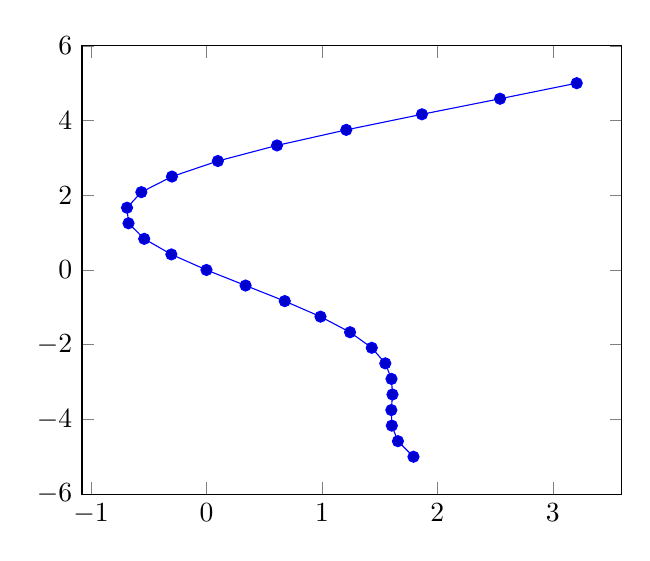
\begin{tikzpicture}
	    \begin{axis}
	        \addplot+[] ({x^2/10-sin(45*x)},{x});
	    \end{axis}
	\end{tikzpicture}
	
\end{image}

\begin{explanation}
As in the previous example, we are looking to determine if there are any values of $x$ for which there are multiple outputs.  Visually, what that means is there are places on the graph that are directly above/below each other. Thinking about this leads to a quick visual “test” to determine if a graph gives $y$ as a function of $x$.

\begin{callout}\textbf{Vertical Line ``Test''}  
Given a graph in the $xy$-plane, if there exists a vertical line that touchs the graph in more than one place, the graph does not represent a function.  If no such vertical line exists, then the relation represented by the graph is also a function.
\end{callout}

Let's use this test to analyze each of the graphs in this example.
\begin{enumerate}[label=\alph*.]
\item  We notice that it is possible to draw a vertical line that touches this graph in two places.

\begin{image}
\begin{tikzpicture}
    \begin{axis}
        \addplot[verticallinetest] coordinates {(-3,-7) (-3,7)};
        \addplot[soliddot] coordinates {(2,4) (-5,-5) (3, 4) (0,4) (4,0) (-3,1) (-3,-2)};
        \addplot[soliddot, color=secondcolor, mark=x, mark options={scale=3}, thick] coordinates {(-3,1) (-3,-2)};
    \end{axis}
\end{tikzpicture}
\end{image}

Therefore, by the vertical line test, this graph is not the graph of a function.  Really, the vertical line we found at $x=-3$ is helping us to quickly identify that both $(-3,-2)$ and $(-3, 1)$ are points on this graph so that for the same input, $3$, there are two different outputs, $-2$ and $1$. 

\item This graph is the graph of a function.  Here are some examples of some vertical lines we might consider.

 \begin{image}
 \begin{tikzpicture}
    \begin{axis}
        \addplot[verticallinetest] coordinates {(-6,-7) (-6,7)};
        \addplot[verticallinetest] coordinates {(-4,-7) (-4,7)};
        \addplot[verticallinetest] coordinates {(-2,-7) (-2,7)};
        \addplot[verticallinetest] coordinates {(2,-7) (2,7)};
        \addplot[verticallinetest] coordinates {(4,-7) (4,7)};
        \addplot[verticallinetest] coordinates {(6,-7) (6,7)};
        \addplot[firstcurve] {0.5*x+2};
        \addplot[hollowdot] coordinates {(-4,0) (2,3) (6, 5)};
        \addplot[soliddot] coordinates {(-4,4) (2,1)};
        \addplot[soliddot, color=secondcolor, mark=x, mark options={scale=3}, thick] coordinates {(-6,-1) (-4,4) (-2,1) (0,2) (2,1) (4,4)};
    \end{axis}
\end{tikzpicture}
 \end{image}
 
 Note that we cannot draw all possible vertical lines.  Really, we only need to look at the points on this graph which are not a line.  We already said the graphs of lines (without any other points or curves above or below that line) are functions.  So on this graph, the interesting points we want to look at more closely are $x=-4$, $x=2$, and $x=6$.  In each of these cases, there is either one or no outputs.  In particular, for $x=-4$ the corresponding output is $y=4$.   There is an open dot at $(-4,0)$ so this point is not in the relation.  Similarly, $(2,1)$ is a point on this graph but $(2,3)$ is not.  At $x=6$, there are no corresponds outputs. We say are function is not defined at $x=6$.
 
 \item
This graph is not a function.  Any vertical line we draw will cross the graph multiple times.  Here is an example of a vertical line at $x=-4$.
 
 \begin{image}
 \begin{tikzpicture}
    \begin{axis}
        \addplot[verticallinetest] coordinates {(-4,-7) (-4,7)};
        \addplot[soliddot, color=secondcolor, mark=x, mark options={scale=3}, thick] coordinates {(-4,6) (-4,3) (-4,-1) (-4,-3) (-4,-5.6)};
        \addplot[firstcurve, samples=29,smooth] {cos(45*x)};
        \addplot[firstcurve, samples=29,smooth] {sin(90*x)+3};
        \addplot[firstcurve, samples=29,smooth] {(cos(45*x))^3-2};
        \addplot[firstcurve, samples=29,smooth] {sqrt(sin(90*x)+1)+5};
        \addplot[firstcurve, samples=29,smooth] {exp(sin(120*x))-6};
    \end{axis}
\end{tikzpicture}
\end{image}

You could consider this a graph of five separate functions all graphed on the same coordinate axes, but that is a different question from the one being asked.  

 \begin{image}
 \begin{tikzpicture}
    \begin{axis}
        \addplot[firstcurve, samples=29,smooth] {cos(45*x)};
        \addplot[secondcurve, samples=29,smooth] {sin(90*x)+3};
        \addplot[thirdcurve, samples=29,smooth] {(cos(45*x))^3-2};
        \addplot[fourthcurve, samples=29,smooth] {sqrt(sin(90*x)+1)+5};
        \addplot[fifthcurve, samples=29,smooth] {exp(sin(120*x))-6};
    \end{axis}
\end{tikzpicture}
\end{image}

\item 
This graph is also not a function.  Even though it is a single curve, it has input values, such as $x=2$ with multiple corresponding output values.

\begin{image}
\begin{tikzpicture}
    \begin{axis}
        \addplot[verticallinetest] coordinates {(2,-7) (2,7)};
        \addplot[soliddot, color=secondcolor, mark=x, mark options={scale=3}, thick] coordinates {(2,4.25) (2,-5.4)};
        \addplot[firstcurve] ({x^2/10-sin(45*x)},{x});
    \end{axis}
\end{tikzpicture}
\end{image}

 \end{enumerate}
\end{explanation}
\end{example}
 
 \subsection{Formula Representation}
 Another common way to represent functions is using a formula.  In the example of Dolbear's Law, the function which models this law is given as a formula by 
 $$D(N)=40+0.25N \text{ for } 50 \leq x \leq 85$$
 When we give functions as a formula, we also need to say which input values are allowed.  In this case, the allowed inputs are $50 \leq x \leq 85$.  If allowed inputs are not given, the inputs are assumed to be all the values for which the formula used to defined the function makes sense.  
 
 Here are some examples of functions represented by a formula.
 
\begin{itemize}
\item $f(x)=x^2$
\item $g(x)=5x-7$
\item $h(x)=\sin(x)$  

Recall that this is the famous function named sine.
\item $z(x)=\frac{x^2\sin(x)-2}{72-x}$
\end{itemize}

Here is an example of working with the formula representation of a function.

\begin{example}
Let $f(x)=5x-2$.  Find $f(1)$.

\begin{explanation}
Recall that the notation $f(1)$ means to evaluate the function $f$ at the input $x=1$.  That is, $f(1)=5(1)-2=3$.
\end{explanation}
\end{example}

\section{Intercepts}
Zero is a very important number, and as we will see later, knowing where a function's $x$- or $y$-value equals zero can be powerful information. 

\begin{definition}[Intercepts]
Say $f$ is a function. 

An \dfn{$x$-intercept} of $f$ is a point $(x,0)$ such that $f(x) = 0$. That is, a point in which the graph of the function touches the $x$-axis. 

The \dfn{$y$-intercept} of $f$ is a point $(0,y)$ such that $f(0) = y$. That is, a point in which the graph of the function touches the $y$-axis. Unlike $x$-intercepts, there can be only one $y$-intercept for each function.
\end{definition}



%\typeout{************************************************}
%\typeout{Summary}
%\typeout{************************************************}

\begin{summary}\begin{itemize}
\item Informally, a function is a process that may be applied to a collection of input values to produce a corresponding collection of output values in such a way that the process produces one and only one output value for any single input value.
\item Formally, a function  is a collection of ordered pairs $(x,y)$ such that any particular value of $x$ is paired with at most one value for $y$. That is, a relation in which each $x$-coordinate is matched with only one $y$-coordinate is said to describe $y$ as a \dfn{function} of $x$.
\item Functions can be used to model many phenomena in the real world, as long as for a given input there is one predictable output.
\item Functions can be represented in many ways including as:
\begin{itemize}
\item sets of ordered pairs
\item tables
\item arrow diagrams
\item graphs
\item formula
\item domain and range
\end{itemize}
\end{itemize}\end{summary}




\end{document}
